% =====================================================================
\chapter{Gravitational waves}\label{ch:gw}
% =====================================================================

\section{Interlude: electrodynamics}

Gravitational waves are best understood in analogy with electromagnetic waves, so we first recall how electrodynamics works (Gaussian units).
\begin{itemize}
\item Electromagnetism is described by the \textbf{Lorentz force} $m\ddot{\vec x}=e\vec E+\frac ec\dot{\vec x}\times\vec B$ and by \textbf{Maxwell's equations}
\[
  \nabla\cdot\vec E=4\pi\rho,\qquad\nabla\times\vec E=-\frac1c\frac{\pd\vec B}{\pd t},\qquad\nabla\cdot\vec B=0,\qquad\nabla\times\vec B=\frac{4\pi}{c}\vec J+\frac1c\frac{\pd\vec E}{\pd t},
\]
with $\rho$ the charge density and $\vec J$ the current density.
\item We typically introduce the \textbf{vector potential} $\vec A$, $\vec B=\nabla\times\vec A$ (which solves $\nabla\cdot\vec B=0$), and the \textbf{scalar potential} $\phi$, $\vec E+\frac1c\frac{\pd\vec A}{\pd t}=-\nabla\phi$ (which solves Faraday's law).
\item The $(4+4)$ equations can be written in a manifestly covariant form, and derived from an action $S=S_m+S_{\rm int}+S_{\rm EM}$ (free particle, interaction, electromagnetic field):
\begin{align*}
  &S_m=-mc\int_\Gamma\sqrt{\dd s^2},\\
  &S_{\rm int}=-\frac ec\int_\Gamma A_\mu\dd x^\mu=-\frac{1}{c^2}\int_\Omega J^\mu A_\mu\,\dd^4\Omega,\\
  &S_{\rm EM}=-\frac{1}{16\pi c}\int_\Omega F^{\mu\nu}F_{\mu\nu}\,\dd^4\Omega,
\end{align*}
where $\Gamma$ is the world-line, $\Omega$ a space-time region, and
\[
  F_{\mu\nu}\equiv\pd_\mu A_\nu-\pd_\nu A_\mu\ \text{(Faraday tensor)},\qquad A^\mu\equiv(\phi,\vec A),\qquad J^\mu\equiv(\rho c,\rho\vec v).
\]
(The overall sign of $S_{\rm int}$ depends on the sign conventions for $A_\mu$.)
\item In particular, the inhomogeneous Maxwell equations read
\begin{equation}
  \pd_\mu F^{\mu\nu}=\frac{4\pi}{c}J^\nu
\end{equation}
(the sign depends on conventions), and they are invariant under \textbf{gauge transformations} $A_\mu(x)\to A'_\mu(x)=A_\mu(x)+\pd_\mu\Lambda(x)$, with $\Lambda$ an arbitrary function, since $F_{\mu\nu}$ is.
\item For example, we can choose $A_\mu$ such that $\pd_\mu A^\mu=0$ (\textbf{Lorenz gauge}). This is always possible: if $\pd_\mu A^\mu\neq0$, choose $\Lambda$ with $\Box\Lambda=-\pd_\mu A^\mu$. In this gauge Maxwell's equations become wave equations, $\Box A^\nu=\frac{4\pi}{c}J^\nu$: in vacuum, electromagnetic waves.
\end{itemize}
\textbf{Why all this?} In GR the same things happen, because the Einstein equations work in every coordinate system: we have the freedom to choose coordinates, and the physics remains unchanged. This freedom plays the role of the gauge freedom of electrodynamics, and with a clever choice (a ``gauge'') the linearised Einstein equations become wave equations.

\section{Linearised gravity}

Same idea as in the Newtonian limit: we expand
\begin{equation}
  g_{\mu\nu}=\eta_{\mu\nu}+h_{\mu\nu},\qquad|h_{\mu\nu}|\ll1 ,
\end{equation}
where $h_{\mu\nu}$ is a perturbation, and we drop all terms of order $h^2$, $(\pd h)^2$, $h\,\pd^2h$, \dots Remember that the inverse metric has a minus sign:
\begin{equation}
  g^{\mu\nu}=\eta^{\mu\nu}-h^{\mu\nu}+\order{h^2}
\end{equation}
(proof: writing $g^{\mu\nu}=\eta^{\mu\nu}+H^{\mu\nu}$, $g_{\mu\nu}g^{\nu\rho}=\delta_\mu{}^\rho+\eta_{\mu\nu}H^{\nu\rho}+h_{\mu\nu}\eta^{\nu\rho}+\order{hH}=\delta_\mu{}^\rho$ requires $H_\mu{}^\rho=-h_\mu{}^\rho$, i.e.\ $H^{\mu\nu}=-h^{\mu\nu}$).

\begin{remarkbox}[Remarks]
\begin{enumerate}[label=(\roman*),nosep]
\item In linearised gravity we raise and lower indices of $h$ (and of all first-order quantities) with $\eta^{\mu\nu}$, $\eta_{\mu\nu}$; the difference with $g$ is of higher order.
\item Summary: $g_{\mu\nu}=\eta_{\mu\nu}+h_{\mu\nu}$, $g^{\mu\nu}=\eta^{\mu\nu}-h^{\mu\nu}$, $g^\mu{}_\nu=\delta^\mu{}_\nu\ (=\eta^\mu{}_\nu)$, where $h^\mu{}_\nu=\eta^{\mu\alpha}h_{\alpha\nu}$ and $h^{\mu\nu}=\eta^{\mu\alpha}\eta^{\nu\beta}h_{\alpha\beta}$; so that $g_{\mu\nu}g^{\nu\rho}=\delta_\mu{}^\rho$ to first order.
\item In linearised gravity, $h_{\mu\nu}$ is a tensor \emph{only under Lorentz transformations} (not under general ones). Under $x'^\mu=L^\mu{}_\nu x^\nu$, $g'_{\mu\nu}=L_\mu{}^\alpha L_\nu{}^\beta(\eta_{\alpha\beta}+h_{\alpha\beta})=\eta_{\mu\nu}+L_\mu{}^\alpha L_\nu{}^\beta h_{\alpha\beta}$, so $h$ transforms as a Lorentz tensor; a general transformation would destroy the split ``background $\eta$ $+$ small perturbation''.
\end{enumerate}
\end{remarkbox}

\paragraph{Gauge transformations.} The split does survive \emph{infinitesimal} coordinate transformations $x'^\mu=x^\mu+\xi^\mu(x)$, with $\xi$ of the same order as $h$. By Problem Sheet 2 (Killing equation), $g'_{\mu\nu}(x')=g_{\mu\nu}(x)-g_{\mu\alpha}\pd_\nu\xi^\alpha-g_{\alpha\nu}\pd_\mu\xi^\alpha$; evaluating both sides at the same coordinate value and dropping second-order terms ($\xi^\alpha\pd_\alpha h$, $h\pd\xi$):
\begin{equation}
  h'_{\mu\nu}=h_{\mu\nu}-\pd_\mu\xi_\nu-\pd_\nu\xi_\mu .
  \label{eq:gauge-h}
\end{equation}
This is the analogue of $A_\mu\to A_\mu+\pd_\mu\Lambda$: $h_{\mu\nu}$ and $h'_{\mu\nu}$ describe the same physical situation.

\section{The Einstein equations in linearised gravity}

\paragraph{Christoffel symbols.} By definition $\Ga{\lambda}{\sigma}{\rho}=\frac12g^{\lambda\mu}(\pd_\sigma g_{\rho\mu}+\pd_\rho g_{\sigma\mu}-\pd_\mu g_{\sigma\rho})$. The bracket contains no $\eta$'s (their derivatives vanish), so it is already linear in $h$ and we can replace $g^{\lambda\mu}\to\eta^{\lambda\mu}$:
\begin{equation}
  \Ga{\lambda}{\sigma}{\rho}\simeq\frac12\eta^{\lambda\mu}\big(\pd_\sigma h_{\rho\mu}+\pd_\rho h_{\sigma\mu}-\pd_\mu h_{\sigma\rho}\big).\tag{1}
\end{equation}
\paragraph{Riemann tensor.} $\Riem{\lambda}{\mu}{\sigma}{\nu}=\pd_\sigma\Ga{\lambda}{\nu}{\mu}-\pd_\nu\Ga{\lambda}{\sigma}{\mu}+\Gamma\Gamma-\Gamma\Gamma$, and the $\Gamma\Gamma$ terms are at least quadratic, $\order{h^2}$, so we remove them:
\begin{equation}
  \Riem{\lambda}{\mu}{\sigma}{\nu}\simeq\pd_\sigma\Ga{\lambda}{\nu}{\mu}-\pd_\nu\Ga{\lambda}{\sigma}{\mu}.\tag{2}
\end{equation}
Inserting (1) in (2):
\begin{align*}
  \Riem{\lambda}{\mu}{\sigma}{\nu}&=\frac12\eta^{\lambda\alpha}\pd_\sigma\big(\pd_\nu h_{\mu\alpha}+\pd_\mu h_{\nu\alpha}-\pd_\alpha h_{\nu\mu}\big)-\frac12\eta^{\lambda\alpha}\pd_\nu\big(\pd_\sigma h_{\mu\alpha}+\pd_\mu h_{\sigma\alpha}-\pd_\alpha h_{\sigma\mu}\big)\\
  &=\frac12\eta^{\lambda\alpha}\big(\pd_\sigma\pd_\mu h_{\nu\alpha}-\pd_\sigma\pd_\alpha h_{\mu\nu}-\pd_\nu\pd_\mu h_{\sigma\alpha}+\pd_\nu\pd_\alpha h_{\mu\sigma}\big),
\end{align*}
since the terms $\pd_\sigma\pd_\nu h_{\mu\alpha}$ cancel. Lowering $\lambda$ with $\eta_{\lambda\alpha}$:
\begin{equation}
  R_{\lambda\mu\sigma\nu}\simeq\frac12\big(\pd_\sigma\pd_\mu h_{\lambda\nu}-\pd_\sigma\pd_\lambda h_{\mu\nu}-\pd_\nu\pd_\mu h_{\lambda\sigma}+\pd_\nu\pd_\lambda h_{\mu\sigma}\big).
\end{equation}
\textit{Comments:} (i) these expressions satisfy the symmetries and the Bianchi identities, with ordinary derivatives instead of covariant ones; (ii) $R_{\lambda\mu\sigma\nu}$ is already $\order h$; (iii) it is \textbf{gauge invariant}: under \eqref{eq:gauge-h} each term changes by third derivatives of $\xi$, which cancel in pairs because partial derivatives commute --- as it should, since curvature is physical.

\paragraph{Ricci tensor.} By definition $R_{\mu\nu}=g^{\lambda\sigma}R_{\lambda\mu\sigma\nu}\simeq\eta^{\lambda\sigma}R_{\lambda\mu\sigma\nu}$ (the correction is $\order{h^2}$):
\begin{equation}
  R_{\mu\nu}\simeq\frac12\big(\pd_\mu\pd^\lambda h_{\nu\lambda}+\pd_\nu\pd^\sigma h_{\sigma\mu}-\Box h_{\mu\nu}-\pd_\mu\pd_\nu h\big),
  \qquad h\equiv\eta^{\mu\nu}h_{\mu\nu},\quad\Box\equiv\eta^{\mu\nu}\pd_\mu\pd_\nu=\frac{1}{c^2}\pd_t^2-\nabla^2 .
\end{equation}
\paragraph{Ricci scalar.} By definition $R=g^{\mu\nu}R_{\mu\nu}\simeq\eta^{\mu\nu}R_{\mu\nu}=\frac12\big(\pd^\nu\pd^\lambda h_{\nu\lambda}+\pd^\mu\pd^\sigma h_{\sigma\mu}-\Box h-\Box h\big)$:
\begin{equation}
  R\simeq\pd^\mu\pd^\nu h_{\mu\nu}-\Box h .
\end{equation}

\paragraph{The Einstein equations.} The general form is $R_{\mu\nu}-\frac12g_{\mu\nu}R=8\pi\GN T_{\mu\nu}$ (we do not consider the $\Lambda$ term, and we set $c=1$). Applying the previous results:
\begin{equation}
  \frac12\big(\pd_\mu\pd^\lambda h_{\nu\lambda}+\pd_\nu\pd^\sigma h_{\sigma\mu}-\Box h_{\mu\nu}-\pd_\mu\pd_\nu h\big)-\frac12\eta_{\mu\nu}\big(\pd^\rho\pd^\sigma h_{\rho\sigma}-\Box h\big)=8\pi\GN T_{\mu\nu}.
  \label{eq:lin-efe-h}
\end{equation}
To simplify this complex equation, we introduce the \textbf{trace-reversed perturbation}
\begin{equation}
  \bar h_{\mu\nu}\equiv h_{\mu\nu}-\frac12\eta_{\mu\nu}h ,\qquad\text{whose trace is}\qquad\bar h\equiv\eta^{\mu\nu}\bar h_{\mu\nu}=h-\frac12\cdot4h=-h
\end{equation}
(hence the name). The relation is easily inverted: $h_{\mu\nu}=\bar h_{\mu\nu}-\frac12\eta_{\mu\nu}\bar h$.

\paragraph{The substitution, step by step.} Using $h_{\mu\nu}=\bar h_{\mu\nu}-\frac12\eta_{\mu\nu}\bar h$ and $h=-\bar h$:
\begin{align*}
  \pd_\mu\pd^\lambda h_{\nu\lambda}&=\pd_\mu\pd^\lambda\bar h_{\nu\lambda}-\tfrac12\pd_\mu\pd_\nu\bar h, &
  \pd_\nu\pd^\sigma h_{\sigma\mu}&=\pd_\nu\pd^\sigma\bar h_{\sigma\mu}-\tfrac12\pd_\nu\pd_\mu\bar h,\\
  \Box h_{\mu\nu}&=\Box\bar h_{\mu\nu}-\tfrac12\eta_{\mu\nu}\Box\bar h, &
  \pd_\mu\pd_\nu h&=-\pd_\mu\pd_\nu\bar h,\\
  \pd^\rho\pd^\sigma h_{\rho\sigma}&=\pd^\rho\pd^\sigma\bar h_{\rho\sigma}-\tfrac12\Box\bar h, &
  \Box h&=-\Box\bar h .
\end{align*}
Hence
\begin{align*}
  R_{\mu\nu}&=\frac12\Big(\pd_\mu\pd^\lambda\bar h_{\nu\lambda}+\pd_\nu\pd^\sigma\bar h_{\sigma\mu}\underbrace{-\pd_\mu\pd_\nu\bar h+\pd_\mu\pd_\nu\bar h}_{=0}-\Box\bar h_{\mu\nu}+\frac12\eta_{\mu\nu}\Box\bar h\Big),\\
  R&=\pd^\rho\pd^\sigma\bar h_{\rho\sigma}-\frac12\Box\bar h+\Box\bar h=\pd^\rho\pd^\sigma\bar h_{\rho\sigma}+\frac12\Box\bar h ,
\end{align*}
and
\[
  R_{\mu\nu}-\frac12\eta_{\mu\nu}R=\frac12\Big(\pd_\mu\pd^\lambda\bar h_{\nu\lambda}+\pd_\nu\pd^\sigma\bar h_{\sigma\mu}-\Box\bar h_{\mu\nu}+\underbrace{\tfrac12\eta_{\mu\nu}\Box\bar h-\tfrac12\eta_{\mu\nu}\Box\bar h}_{=0}-\eta_{\mu\nu}\pd^\rho\pd^\sigma\bar h_{\rho\sigma}\Big).
\]
\begin{keyresult}[Linearised Einstein equations]
\begin{equation}
  \pd_\mu\pd^\lambda\bar h_{\nu\lambda}+\pd_\nu\pd^\sigma\bar h_{\sigma\mu}-\Box\bar h_{\mu\nu}-\eta_{\mu\nu}\pd^\rho\pd^\sigma\bar h_{\rho\sigma}=16\pi\GN T_{\mu\nu}.
  \label{eq:lin-efe}
\end{equation}
\end{keyresult}
So far, we have introduced the most important results to study gravitational waves in the approximation of weak fields.

\section{The harmonic gauge}

Interestingly, linearised gravity does by no means uniquely specify the perturbation $h_{\mu\nu}$: the freedom to perform an infinitesimal coordinate transformation $x\to x'=x+\xi(x)$ gives rise to the \emph{gauge transformations} \eqref{eq:gauge-h}. Remember that in electrodynamics we introduce the Lorenz gauge $\pd_\mu A^\mu=0$. Analogously, we choose to work in the \textbf{harmonic} (or Hilbert, or de Donder) \textbf{gauge}:
\begin{equation}
  \boxed{\pd^\mu\bar h_{\mu\nu}=0}.
\end{equation}
(We go to the coordinate system in which $\bar h_{\mu\nu}$ has this form.) In this gauge the first, second and fourth terms of \eqref{eq:lin-efe} vanish, and the EFE become
\begin{equation}
  \boxed{\Box\bar h_{\mu\nu}=-16\pi\GN T_{\mu\nu}}\qquad\Big(=-\frac{16\pi\GN}{c^4}T_{\mu\nu}\Big).
\end{equation}
Thus $\bar h_{\mu\nu}$ represents a quantity that propagates as a wave at the vacuum speed of light, on a flat Minkowski background, and which is sourced by the energy--momentum tensor $T_{\mu\nu}$ of matter: in other words, $\bar h_{\mu\nu}$ is a \textbf{gravitational wave}.

\paragraph{Can we always reach the harmonic gauge?} Under \eqref{eq:gauge-h}, $h'=h-2\pd\cdot\xi$ and
\[
  \bar h'_{\mu\nu}=\bar h_{\mu\nu}-\pd_\mu\xi_\nu-\pd_\nu\xi_\mu+\eta_{\mu\nu}\pd^\alpha\xi_\alpha
  \quad\Longrightarrow\quad\pd^\mu\bar h'_{\mu\nu}=\pd^\mu\bar h_{\mu\nu}-\Box\xi_\nu-\pd_\nu\pd^\mu\xi_\mu+\pd_\nu\pd^\alpha\xi_\alpha=\pd^\mu\bar h_{\mu\nu}-\Box\xi_\nu .
\]
So choosing $\xi$ as a solution of $\Box\xi_\nu=\pd^\mu\bar h_{\mu\nu}$ (always possible: it is a wave equation with a source) brings us to the harmonic gauge. N.B.: if we are already in the harmonic gauge, a further transformation with $\Box\xi_\nu=0$ keeps us in the harmonic gauge (\emph{residual gauge freedom}).

\paragraph{Formal solution.} As in electrodynamics, the solution of the wave equation with the correct (causal) boundary conditions is the \emph{retarded} solution (the Green function of $\Box=\pd_t^2-\nabla^2$ gives $\psi=\int\frac{f(t-|\vec x-\vec x'|,\vec x')}{|\vec x-\vec x'|}\dd^3x'$ for $\Box\psi=4\pi f$):
\begin{equation}
  \bar h_{\mu\nu}(t,\vec x)=-4\GN\int\dd^3x'\,\frac{T_{\mu\nu}(t-|\vec x-\vec x'|,\vec x')}{|\vec x-\vec x'|}.
  \label{eq:retarded}
\end{equation}
The source is evaluated at the \emph{retarded time} $t-|\vec x-\vec x'|$ (the perturbation travels at the speed of light). (In the signature $(-,+,+,+)$, where $\Box=-\pd_t^2+\nabla^2$, the same physics is written $\Box\bar h_{\mu\nu}=-16\pi\GN T_{\mu\nu}$, $\bar h_{\mu\nu}=+4\GN\int T_{\mu\nu}/|\vec x-\vec x'|$; the sign difference just reflects $\eta\to-\eta$.) \textit{Check:} for a static non-relativistic source, $\bar h_{00}=-4\GN\int\frac{\rho}{|\vec x-\vec x'|}=4\Phi$, $\bar h=\bar h_{00}$, so $h_{00}=\bar h_{00}-\frac12\bar h=2\Phi$: the Newtonian limit $g_{00}=1+2\Phi$ is recovered.

\section{The transverse--traceless (TT) gauge}

$\bar h_{\mu\nu}$ is symmetric, so it has a priori $10$ independent components. The harmonic gauge condition (4 equations) reduces them to $6$. This means that the harmonic gauge condition does not uniquely specify the metric perturbation: indeed, any gauge transformation whose generator satisfies $\Box\xi_\mu=0$ preserves the gauge condition. To uniquely specify the metric perturbation, $4$ additional conditions can be imposed (one for each $\xi_\mu$), leaving $\boxed{2}$ independent, physical components (polarisations).

\paragraph{In practice (in vacuum).} Outside the sources $\Box\bar h_{\mu\nu}=0$, and we can use the residual freedom $\Box\xi_\mu=0$:
\begin{enumerate}
\item choose $\xi^0$ such that $\bar h=0$, i.e.\ $\bar h_{\mu\nu}$ is traceless (then $\bar h_{\mu\nu}=h_{\mu\nu}$);
\item choose the $\xi^i$ such that $h_{0i}=0$.
\end{enumerate}
Then the $\nu=0$ component of the harmonic condition gives $\pd^\mu h_{\mu0}=\pd^0h_{00}=0$: $h_{00}$ is time independent. A time-independent $h_{00}$ is just a static Newtonian field (as in \cref{ch:efe}), which does not describe a wave; for the wave part we set $h_{00}=0$. We are left with
\begin{equation}
  \boxed{h_{0\mu}=0,\qquad h=\eta^{\mu\nu}h_{\mu\nu}=0\ (\text{traceless}),\qquad\pd^jh_{ij}=0\ (\text{transverse})}.
\end{equation}
This is the \textbf{transverse--traceless gauge}, and we write $h^{\rm TT}_{\mu\nu}$.

\begin{remarkbox}[N.B.]
In vacuum ($\Box\bar h_{\mu\nu}=0$) one can always choose $\Box\xi_\mu=0$ appropriately, and the TT gauge is always possible. With matter ($\Box\bar h_{\mu\nu}\neq0$) it is not always possible to go to the TT gauge.
\end{remarkbox}

\paragraph{A convention for the spatial components.} With our signature $\eta_{ij}=-\delta_{ij}$, so $g_{ij}=-\delta_{ij}+h_{ij}$ and the proper spatial distance is $\dd l^2=(\delta_{ij}-h_{ij})\dd x^i\dd x^j$. To agree with the usual GW literature (written in $(-,+,+,+)$), from now on we denote by $h^{\rm TT}_{ij}$ the spatial \emph{strain}, i.e.\ the perturbation of the spatial metric $\dd l^2=(\delta_{ij}+h^{\rm TT}_{ij})\dd x^i\dd x^j$; in terms of the components of $h_{\mu\nu}=g_{\mu\nu}-\eta_{\mu\nu}$ this is $h^{\rm TT}_{ij}=-h_{ij}=h^i{}_j$. Since all equations are linear, $\Box h^{\rm TT}_{ij}=0$, transversality and tracelessness are unaffected.

\section{Propagation in vacuum: plane waves}

In vacuum,
\begin{equation}
  \Box h^{\rm TT}_{\mu\nu}=0 :
\end{equation}
it is a \textbf{wave equation}. We look for plane-wave solutions
\begin{equation}
  h^{\rm TT}_{\mu\nu}=\varepsilon_{\mu\nu}\,e^{ik_\alpha x^\alpha}\quad(\text{real part understood}),\qquad k^\mu=(\omega,\vec k),
\end{equation}
where $\varepsilon_{\mu\nu}$ is the (constant, symmetric) \emph{polarisation tensor}. Then:
\begin{itemize}
\item $\Box h=-k_\alpha k^\alpha h=0\Rightarrow k_\alpha k^\alpha=\omega^2-|\vec k|^2=0$: $\omega=|\vec k|$ (dispersion relation). The wave vector is null: \textbf{gravitational waves travel at the speed of light}.
\item Harmonic (transverse) condition: $k^\mu\varepsilon_{\mu\nu}=0$; TT: $\varepsilon_{0\mu}=0$, $\varepsilon^\mu{}_\mu=0$.
\end{itemize}
For propagation in the $z$-direction, $k^\mu=\omega(1,0,0,1)$, transversality gives $k^\mu\varepsilon_{\mu\nu}=\omega(\varepsilon_{0\nu}+\varepsilon_{3\nu})=0\Rightarrow\varepsilon_{3\nu}=0$; with $\varepsilon_{0\nu}=0$ and tracelessness, $\varepsilon_{22}=-\varepsilon_{11}$. Only two independent components remain, $h_+$ and $h_\times$:
\begin{equation}
  h^{\rm TT}_{\alpha\beta}=\begin{pmatrix}0&0&0&0\\0&h_+&h_\times&0\\0&h_\times&-h_+&0\\0&0&0&0\end{pmatrix}\cos\Big[\omega\Big(t-\frac zc\Big)\Big],
\end{equation}
where $h_+$, $h_\times$ are the amplitudes of the two polarisation modes (``plus'' and ``cross''). We can also write
\[
  h^{\rm TT}_{ij}=h_+\,\varepsilon^+_{ij}\cos[\omega(t-z/c)]+h_\times\,\varepsilon^\times_{ij}\cos[\omega(t-z/c)],\qquad
  \varepsilon^+=\begin{pmatrix}1&0&0\\0&-1&0\\0&0&0\end{pmatrix},\quad\varepsilon^\times=\begin{pmatrix}0&1&0\\1&0&0\\0&0&0\end{pmatrix}.
\]
Then the \textbf{line element} is
\begin{equation}
  \dd s^2=c^2\dd t^2-(1+h_+\cos\varphi)\dd x^2-(1-h_+\cos\varphi)\dd y^2-2h_\times\cos\varphi\,\dd x\,\dd y-\dd z^2,\qquad\varphi\equiv\omega\Big(t-\frac zc\Big).
\end{equation}

\section{Effects of gravitational waves on test particles}

\paragraph{1) A single free particle in the path of a GW.} A free particle obeys the geodesic equation $\ddot x^\mu+\Ga{\mu}{\nu}{\rho}\dot x^\nu\dot x^\rho=0$. Take a particle initially at rest at $\tau=0$: $\frac{\dd x^i}{\dd\tau}=0$. Then
\[
  \ddot x^\mu=-\Ga{\mu}{0}{0}\Big(\frac{\dd x^0}{\dd\tau}\Big)^2,\qquad\Ga{\mu}{0}{0}=\frac12\eta^{\mu\sigma}\big(\pd_0h_{0\sigma}+\pd_0h_{0\sigma}-\pd_\sigma h_{00}\big).
\]
In the TT gauge $h_{0\mu}=0$, so $\Ga{\mu}{0}{0}=0$ and $\ddot x^\mu=0$ (at $\tau=0$, and hence at all times): the particle stays at rest, i.e.\ at constant TT coordinates. \textbf{But} ``at rest'' with respect to its coordinate system: the TT coordinates are attached to the freely-falling particles themselves. To see a physical effect, we must consider the \emph{proper distance} between two particles.

\paragraph{2) Two particles at $(x_0,0,0)$ and $(-x_0,0,0)$.} How does the proper distance evolve? For a wave travelling along $z$ (at $z=0$), with the particles at fixed coordinates,
\begin{align}
  \Delta l&=\int_{-x_0}^{x_0}\sqrt{|\dd s^2|}=\int_{-x_0}^{x_0}\sqrt{|g_{xx}|}\,\dd x=\int_{-x_0}^{x_0}\sqrt{1+h_+\cos(\omega t)}\,\dd x\nonumber\\
  &\simeq L_0\Big[1+\frac12h_+\cos(\omega t)\Big],\qquad L_0=2x_0,
\end{align}
where we Taylor-expanded $\sqrt{1+\epsilon}\simeq1+\epsilon/2$. N.B.: for two particles at $(0,\pm x_0,0)$ instead, $\Delta l=L_0\big[1-\frac12h_+\cos(\omega t)\big]$.

\textit{Comments:}
\begin{enumerate}
\item The proper distance \emph{does} change, periodically, with the frequency of the wave: stretched along $x$ while squeezed along $y$, and vice versa half a period later.
\item $\Delta L\equiv\Delta l-L_0\propto L_0$ (the initial separation): the effect is a \emph{strain} $\Delta L/L_0=\frac12h_+\cos\omega t$. Since $h\sim10^{-21}$ for typical astrophysical sources, gravitational-wave detectors must be large (LIGO/Virgo arms are $3$--$4$\,km long, and measure $\Delta L\sim10^{-18}$\,m).
\item If you rotate the system by $45^\circ$, you get the same answer but with $h_\times$: the two polarisations differ by a $45^\circ$ rotation.
\item The effect on a ring of particles in the $xy$ plane is shown in \cref{fig:ring}. There is no effect along the direction of propagation: the waves are \emph{transverse}.
\end{enumerate}

\begin{figure}[ht]
\centering
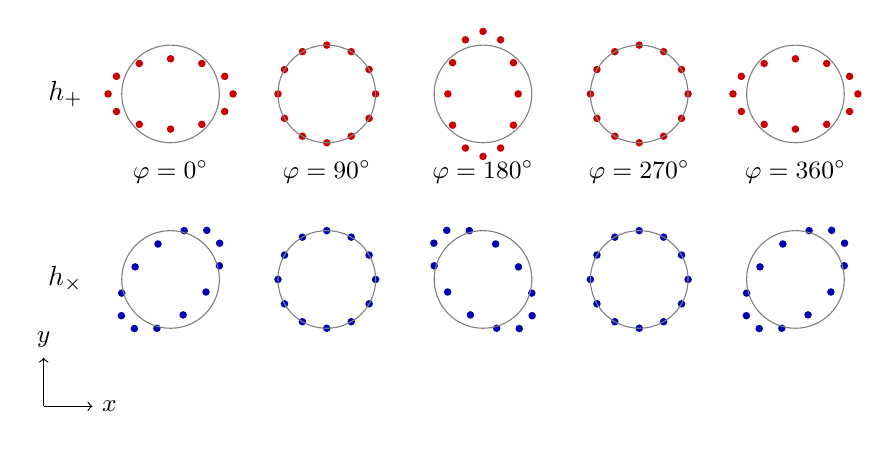
\begin{tikzpicture}[scale=0.62]
  \foreach \i/\ph in {0/0,1/90,2/180,3/270,4/360}{
    \begin{scope}[shift={(3.2*\i,0)}]
      \pgfmathsetmacro{\e}{0.28*cos(\ph)}
      \foreach \t in {0,30,...,330}{\fill[red!80!black] ({(1+\e)*cos(\t)},{(1-\e)*sin(\t)}) circle (2.2pt);}
      \draw[gray,thin] (0,0) circle (1);
      \node at (0,-1.6) {\small $\varphi=\ph^\circ$};
    \end{scope}
    \begin{scope}[shift={(3.2*\i,-3.8)}]
      \pgfmathsetmacro{\e}{0.28*cos(\ph)}
      \foreach \t in {0,30,...,330}{
        \pgfmathsetmacro{\X}{cos(\t)}\pgfmathsetmacro{\Y}{sin(\t)}
        \fill[blue!70!black] ({\X+\e*\Y},{\Y+\e*\X}) circle (2.2pt);}
      \draw[gray,thin] (0,0) circle (1);
    \end{scope}}
  \node[left] at (-1.6,0) {$h_+$};
  \node[left] at (-1.6,-3.8) {$h_\times$};
  \draw[->] (-2.6,-6.4) -- (-1.6,-6.4) node[right] {\small $x$};
  \draw[->] (-2.6,-6.4) -- (-2.6,-5.4) node[above] {\small $y$};
\end{tikzpicture}
\caption{Effect of a gravitational wave propagating along $z$ on a ring of free test particles in the $xy$ plane, over one period ($\varphi=\omega t$). Top: plus polarisation $h_+$ (the ring is alternately stretched along $x$ and squeezed along $y$, and vice versa). Bottom: cross polarisation $h_\times$ (the same pattern rotated by $45^\circ$). The deformation is enormously exaggerated.}
\label{fig:ring}
\end{figure}

\section{Generation of gravitational waves: Einstein's quadrupole formula}

We now describe the generation of gravitational waves by isolated systems. For each component of $\bar h_{\mu\nu}$ the linear equation can be solved by \eqref{eq:retarded} (in the harmonic gauge).

\paragraph{Compact source, far away.} Assume a compact source observed from far away: $|\vec x-\vec x'|\simeq|\vec x|\equiv r$ for all points $\vec x'$ of the source (and, for slowly moving sources, the retardation across the source can be neglected). Then
\begin{equation}
  \bar h_{\mu\nu}(t,r)\simeq-\frac{4\GN}{r}\int\dd^3x'\,T_{\mu\nu}(t-r,\vec x').
\end{equation}
In linearised theory $h_{\mu\nu}$ and $T_{\mu\nu}$ are of the same order (Einstein equations), so the conservation law $D_\mu T^{\mu\nu}=0$ reduces to $\pd_\mu T^{\mu\nu}=0$ at this order. Starting from this, one can play around with the components ($c=1$; all integrals over a volume $V$ containing the source, on whose boundary $T^{\mu\nu}=0$).

\paragraph{1. $\nu=0$ and $\nu=i$: conserved quantities.} $\pd_\mu T^{\mu0}=0\Rightarrow\pd_0T^{00}=-\pd_kT^{k0}$. Integrating over the region where $T^{\mu\nu}\neq0$, by Gauss' theorem
\[
  \frac{\pd}{\pd t}\int_VT^{00}\dd^3x=-\int_V\pd_kT^{k0}\dd^3x=-\oint_{\pd V}T^{k0}\dd\Sigma_k=0 .
\]
So $\int T^{00}\dd^3x$ is constant (total energy/mass), and similarly $\int T^{0i}\dd^3x$ (total momentum). Hence $\bar h^{0\nu}$ is constant in time: it is the static (Newtonian) part of the field and it does not contribute to the waves; we decide to put $\bar h^{0\nu}=0$ for the radiative part.

\paragraph{2. Integrals of $T^{ij}$.} $\pd_\mu T^{\mu i}=0\Rightarrow\pd_0T^{0i}=-\pd_kT^{ki}$. Multiply by $x^j$ and integrate, integrating by parts:
\begin{align*}
  \frac{\pd}{\pd t}\int_Vx^jT^{0i}\dd^3x&=-\int_Vx^j\pd_kT^{ki}\dd^3x=-\int_V\pd_k\big(x^jT^{ki}\big)\dd^3x+\int_VT^{ki}\frac{\pd x^j}{\pd x^k}\dd^3x\\
  &=-\oint_{\pd V}x^jT^{ki}\dd\Sigma_k+\int_VT^{ji}\dd^3x=\int_VT^{ij}\dd^3x ,
\end{align*}
since $T$ vanishes on the boundary and $\pd x^j/\pd x^k=\delta^j{}_k$. But $T^{\mu\nu}$ is symmetric, so we get the same result with $i\leftrightarrow j$. Adding the two:
\begin{equation}
  \frac{\pd}{\pd t}\int_V\big(T^{i0}x^j+T^{j0}x^i\big)\dd^3x=2\int_VT^{ij}\dd^3x .\tag{$\star$}
\end{equation}
\paragraph{3. Second moment of $T^{00}$.} $\pd_\mu T^{\mu0}=0\Rightarrow\pd_0T^{00}=-\pd_kT^{k0}$. Multiply by $x^ix^j$ and integrate by parts:
\[
  \int_Vx^ix^j\pd_0T^{00}\dd^3x=-\int_Vx^ix^j\pd_kT^{k0}\dd^3x=\int_VT^{k0}\frac{\pd(x^ix^j)}{\pd x^k}\dd^3x=\int_V\big(T^{i0}x^j+T^{j0}x^i\big)\dd^3x .
\]
Hence $\frac{\pd}{\pd t}\int x^ix^jT^{00}=\int(T^{i0}x^j+T^{j0}x^i)$, and differentiating once more and using ($\star$):
\begin{equation}
  \frac{\pd^2}{\pd t^2}\int_Vx^ix^jT^{00}\dd^3x=2\int_VT^{ij}\dd^3x .
\end{equation}

\begin{definition}{Quadrupole moment of the source}{quadrupole}
\begin{equation}
  Q^{ij}(t)\equiv\int_VT^{00}(t,\vec x)\,x^ix^j\,\dd^3x ,\qquad\ddot Q^{ij}\equiv\frac{\pd^2Q^{ij}}{\pd t^2}.
\end{equation}
\end{definition}
Therefore $\int T^{ij}\dd^3x=\frac12\ddot Q^{ij}$ and the solution of the linearised EFE is
\begin{equation}
  \bar h_{\mu0}=0,\qquad\bar h_{ij}=-\frac{2\GN}{r}\ddot Q_{ij}(t-r)\quad\Longleftrightarrow\quad\text{strain}\ \ \frac{2\GN}{r}\ddot Q_{ij}(t-r)
\end{equation}
(using the strain convention of the previous section, $\bar h^{\rm strain}_{ij}=-\bar h_{ij}$). Note: if the source has spherical symmetry, $Q_{ij}\propto\delta_{ij}$ with $\ddot Q_{ij}$ pure trace, which is removed by the TT projection below: spherically symmetric collapses or pulsations do not emit gravitational waves (in agreement with Birkhoff's theorem).

\paragraph{Comparison with electromagnetism.} In electrodynamics the leading radiation is \emph{dipole} radiation, $\propto\ddot{\vec d}$ with $\vec d=\int\rho_e\vec x$. The gravitational analogue, the mass dipole $\int T^{00}\vec x$, is (proportional to) the position of the centre of mass, whose second derivative vanishes by momentum conservation (item 1 above). Likewise the ``magnetic dipole'' analogue is the conserved angular momentum. Hence the leading gravitational radiation is \textbf{quadrupolar}, which is much weaker.

\paragraph{Moving to the TT gauge.} We now want to preserve the harmonic gauge while switching to the TT gauge. For a wave travelling radially, along $\vec n=\vec x/r$:
\begin{itemize}[nosep]
\item already $\bar h_{\mu0}=0$;
\item traceless condition: $\delta^{ij}h^{\rm TT}_{ij}=0$;
\item transverse condition: $n^ih^{\rm TT}_{ij}=0$.
\end{itemize}
In order to do that we introduce the projector
\begin{equation}
  P_{ij}\equiv\delta_{ij}-n_in_j ,
\end{equation}
which is symmetric and projects vectors onto the plane transverse to $\vec n$: $P_{ij}n^j=n_i-n_in_jn^j=n_i-n_i=0$, and $P_{ik}P_{kj}=P_{ij}$ (it is a projector); its trace is $P_{ii}=3-1=2$. We then introduce
\begin{equation}
  \Lambda_{ij,k\ell}\equiv P_{ik}P_{j\ell}-\frac12P_{ij}P_{k\ell},\qquad h^{\rm TT}_{ij}=\Lambda_{ij,k\ell}\,\bar h_{k\ell}.
\end{equation}
\begin{exercise}{$h^{\rm TT}_{ij}$ is transverse and traceless}{tt-proof}
\textit{Transverse:} $n^ih^{\rm TT}_{ij}=\big(n^iP_{ik}P_{j\ell}-\frac12n^iP_{ij}P_{k\ell}\big)\bar h_{k\ell}=0$, since $n^iP_{ik}=0$ and $n^iP_{ij}=0$.

\textit{Traceless:} $\delta^{ij}h^{\rm TT}_{ij}=\big(P_{ik}P_{i\ell}-\frac12P_{ii}P_{k\ell}\big)\bar h_{k\ell}=\big(P_{k\ell}-\frac12\cdot2\,P_{k\ell}\big)\bar h_{k\ell}=0$, using $P_{ik}P_{i\ell}=P_{k\ell}$ (projector) and $P_{ii}=2$.

Moreover $\Lambda$ is itself a projector ($\Lambda_{ij,k\ell}\Lambda_{k\ell,mn}=\Lambda_{ij,mn}$), so applying it to a tensor that is already TT leaves it unchanged.
\end{exercise}

\begin{keyresult}[Einstein's quadrupole formula]
In the end:
\begin{equation}
  h^{\rm TT}_{\mu0}=0,\qquad h^{\rm TT}_{ij}(t,\vec x)=\frac{2\GN}{c^4r}\,\ddot Q^{\rm TT}_{ij}\Big(t-\frac rc\Big),\qquad Q^{\rm TT}_{ij}=\Lambda_{ij,k\ell}\,Q_{k\ell}.
\end{equation}
\end{keyresult}

\section{Example: a binary system in a circular orbit}

Consider two masses $m_1$, $m_2$ in a circular orbit around their centre of mass (CM), in the $xy$ plane (\cref{fig:binary}). Let $M=m_1+m_2$, $R=r_1+r_2$ the separation, and $\mu=m_1m_2/M$ the reduced mass. With the CM at the origin, $m_1\vec r_1+m_2\vec r_2=0$, so $r_1=\frac{m_2}{M}R$, $r_2=\frac{m_1}{M}R$.

\begin{figure}[ht]
\centering
\begin{tikzpicture}[scale=1.1,>=Stealth]
  \draw[->] (-2.2,0) -- (2.4,0) node[right] {$x$};
  \draw[->] (0,-1.8) -- (0,2.0) node[above] {$y$};
  \draw[dashed,gray] (0,0) circle (0.7);
  \draw[dashed,gray] (0,0) circle (1.4);
  \fill[blue!70!black] (40:0.7) circle (4pt); \node[blue!70!black] at (0.82,0.22) {$m_1$};
  \fill[red!70!black] (220:1.4) circle (3pt) node[below left] {$m_2$};
  \draw[thick] (220:1.4) -- (40:0.7);
  \node[font=\small] at (0.17,0.36) {$r_1$};
  \node[font=\small] at (-0.42,-0.62) {$r_2$};
  \draw[->,thick] (40:0.7) -- ++(130:0.6);
  \draw[->,thick] (220:1.4) -- ++(310:0.6);
  \draw[->] (1.15,0) arc (0:40:1.15); \node[font=\small] at (1.5,0.42) {$\Omega t$};
  \node[align=left,font=\small] at (3.6,1.3) {$M=m_1+m_2$\\$R=r_1+r_2$\\ observer on the $z$ axis};
\end{tikzpicture}
\caption{A binary system in a circular orbit in the $xy$ plane, around its centre of mass at the origin. The observer is located far away on the $z$ axis.}
\label{fig:binary}
\end{figure}

\paragraph{1) Newtonian orbit.} The gravitational force provides the centripetal force:
\[
  \frac{\GN m_1m_2}{R^2}=m_1\Omega^2r_1=m_1\Omega^2\frac{m_2}{M}R\quad\Longrightarrow\quad\Omega^2=\frac{\GN M}{R^3}\quad\text{(Kepler's third law)}.
\]
\paragraph{2) Trajectories.}
\[
  \vec x_1=\begin{pmatrix}r_1\cos\Omega t\\ r_1\sin\Omega t\\0\end{pmatrix},\qquad
  \vec x_2=\begin{pmatrix}-r_2\cos\Omega t\\ -r_2\sin\Omega t\\0\end{pmatrix}.
\]
\paragraph{3) Quadrupole moment.} For point masses (non-relativistic) $T^{00}=\sum_{a=1}^2m_ac^2\,\delta(x-x_a)\delta(y-y_a)\delta(z)$ (we set $c=1$ below), so that
\[
  Q^{ij}(t)=\int_VT^{00}(t,\vec x)x^ix^j\dd^3x=\sum_am_a\,x_a^i(t)\,x_a^j(t).
\]
For instance, using $m_1r_1^2+m_2r_2^2=\frac{m_1m_2^2+m_2m_1^2}{M^2}R^2=\mu R^2$:
\[
  Q_{xx}=m_1x_1^2+m_2x_2^2=\mu R^2\cos^2\Omega t=\frac{\mu R^2}{2}\cos2\Omega t+\text{const},
\]
and similarly $Q_{yy}=\mu R^2\sin^2\Omega t=-\frac{\mu R^2}2\cos2\Omega t+\text{const}$, $Q_{xy}=\mu R^2\sin\Omega t\cos\Omega t=\frac{\mu R^2}{2}\sin2\Omega t$, $Q_{iz}=0$. In the end
\begin{equation}
  Q_{ij}=\frac{\mu R^2}{2}\begin{pmatrix}\cos2\Omega t&\sin2\Omega t&0\\ \sin2\Omega t&-\cos2\Omega t&0\\0&0&0\end{pmatrix}+\text{const},
  \qquad\ddot Q_{ij}=-2\mu R^2\Omega^2\begin{pmatrix}\cos2\Omega t&\sin2\Omega t&0\\ \sin2\Omega t&-\cos2\Omega t&0\\0&0&0\end{pmatrix}.
\end{equation}
\paragraph{4) TT projection.} Assume the observer is along the $z$ axis: unit vector $\vec n=(0,0,1)$ and projector $P_{ij}=\delta_{ij}-n_in_j=\mathrm{diag}(1,1,0)$. Then, e.g.,
\[
  Q^{\rm TT}_{xx}=\Lambda_{xx,k\ell}Q_{k\ell}=\Big(P_{xk}P_{x\ell}-\frac12P_{xx}P_{k\ell}\Big)Q_{k\ell}=\Big(P_{xx}^2-\frac12P_{xx}^2\Big)Q_{xx}-\frac12P_{xx}P_{yy}Q_{yy}=\frac12(Q_{xx}-Q_{yy}),
\]
and similarly $Q^{\rm TT}_{yy}=-\frac12(Q_{xx}-Q_{yy})$, $Q^{\rm TT}_{xy}=Q_{xy}$, $Q^{\rm TT}_{iz}=0$:
\[
  Q^{\rm TT}_{ij}=\begin{pmatrix}\frac12(Q_{xx}-Q_{yy})&Q_{xy}&0\\ Q_{xy}&-\frac12(Q_{xx}-Q_{yy})&0\\0&0&0\end{pmatrix}.
\]
(For this particular source $Q_{ij}$ restricted to the $xy$ plane is already traceless up to a constant, so the projection only removes the constant part.)

\paragraph{5) The waveform.} So $h^{\rm TT}_{\mu0}=0$ and $h^{\rm TT}_{ij}=\frac{2\GN}{r}\ddot Q^{\rm TT}_{ij}(t-r)$, which has exactly the plane-wave form of the previous sections with $r=z$:
\begin{equation}
  h^{\rm TT}_{\mu\nu}=\begin{pmatrix}0&0&0&0\\0&h_+&h_\times&0\\0&h_\times&-h_+&0\\0&0&0&0\end{pmatrix},
\end{equation}
\begin{keyresult}[Gravitational waves from a circular binary (observer on the axis)]
\begin{equation}
  h_+(t)=-\frac{4\GN\mu R^2\Omega^2}{c^4z}\cos\Big[2\Omega\Big(t-\frac zc\Big)\Big],\qquad
  h_\times(t)=-\frac{4\GN\mu R^2\Omega^2}{c^4z}\sin\Big[2\Omega\Big(t-\frac zc\Big)\Big].
\end{equation}
\end{keyresult}
\textit{Comments:} the waves have \textbf{twice the orbital frequency} ($\omega_{\rm GW}=2\Omega$), since the mass distribution returns to the same configuration after half an orbit; the two polarisations are out of phase by $\pi/2$ (circular polarisation, for an observer on the axis); the amplitude decreases as $1/r$. Using Kepler's law, $\mu R^2\Omega^2=\mu(\GN M\Omega)^{2/3}$, and for a typical stellar-mass binary at $\sim100$\,Mpc one gets $h\sim10^{-21}$--$10^{-22}$. The energy carried away by these waves makes the orbit shrink (as observed in the Hulse--Taylor binary pulsar), until the two objects merge: the signals detected by LIGO/Virgo since 2015.
